\documentclass[letterpaper, 11pt]{article}
\usepackage[margin=1in]{geometry}

% Set the typeface to Times Roman
\usepackage{times}

%\usepackage{hyperref}
\usepackage{amsfonts}%
\usepackage{amssymb}%
\usepackage{amsthm}% allows theoremstyles (see below) and provides a proof environment
\usepackage{bm}
\usepackage{relsize}
\usepackage{graphicx}
\usepackage{caption}
\usepackage{epstopdf}
\usepackage{amsmath}
\usepackage{tikz}
\usetikzlibrary{trees,arrows}
\usetikzlibrary{decorations}
\usetikzlibrary[decorations]
\usepgflibrary{decorations.pathmorphing}
\usepgflibrary[decorations.pathmorphing]
\usetikzlibrary{decorations.pathmorphing}
\usetikzlibrary[decorations.pathmorphing]
\usepackage{booktabs}
\usepackage[authoryear]{natbib}
\usepackage{subcaption}
\usepackage{algorithm}
\usepackage[noend]{algpseudocode}
\usepackage{pseudocode}
%\usepackage{float}
\usepackage{verbatim} %% for commenting blocks
\usepackage[authoryear]{natbib}
\usepackage{url}

\bibpunct{(}{)}{,}{}{}{;} %% added this to make \citep{x} use parentheses

\newcommand{\problemAnswer}[1]{%#1% Defines the problem answer command with the content as the only argument
\noindent\framebox[0.95\columnwidth][c]{\begin{minipage}{0.92\columnwidth}\color{blue}{#1}\end{minipage}} % Makes the box around the problem answer and puts the content inside
}

%% independence symbol and expectation operator %%
\newcommand\independent{\protect\mathpalette{\protect\independenT}{\perp}}
\def\independenT#1#2{\mathrel{\rlap{$#1#2$}\mkern2mu{#1#2}}}

\DeclareMathOperator{\circlearrow}{\hbox{$\circ$}\kern-1.5pt\hbox{$\rightarrow$}}
\DeclareMathOperator{\circlecircle}{\hbox{$\circ$}\kern-1.2pt\hbox{$--$}\kern-1.5pt\hbox{$\circ$}}

\DeclareMathOperator{\an}{an}
\DeclareMathOperator{\pa}{pa}
\DeclareMathOperator{\ch}{ch}
\DeclareMathOperator{\pre}{pre}
\DeclareMathOperator{\de}{de}
\DeclareMathOperator{\nd}{nd}
\DeclareMathOperator{\sib}{sib}
\DeclareMathOperator{\dis}{dis}
\DeclareMathOperator{\mb}{mb}
\DeclareMathOperator{\omb}{omb}
\DeclareMathOperator{\doo}{do}
\DeclareMathOperator{\odds}{\text{OR}}
\DeclareMathOperator*{\argmax}{arg\,max}
\DeclareMathOperator*{\argmin}{arg\,min}
\definecolor{lemon}{RGB}{ 242, 200,  24}
\def\ci{\perp\!\!\!\perp}
\newcommand{\E}{\mathbb{E}}
\newcommand{\G}{\mathcal{G}}

\newcommand\indep{\protect\mathpalette{\protect\independenT}{\perp}}
\def\independenT#1#2{\mathrel{\rlap{$#1#2$}\mkern2mu{#1#2}}}

\newtheorem{Lma}{Lemma}
\newtheorem{Thm}{Theorem}

\DeclareMathOperator{\diedgeright}{\textcolor{blue}{\boldsymbol{\rightarrow}}}
\DeclareMathOperator{\diedgeleft}{\textcolor{blue}{\boldsymbol{\leftarrow}}}
\DeclareMathOperator{\biedge}{\textcolor{red}{\boldsymbol{\leftrightarrow}}}
\DeclareMathOperator{\udedge}{\textcolor{brown}{\boldsymbol{\textendash}}}
%%%%%%%%%%%%%%%%%%%%%%%%%%%%

\title{Final Project Proposal}

\author{Josh Popp}

\date{Mar 23, 2021}

\begin{document}

\maketitle

\setlength{\parindent}{0em}
\setlength{\parskip}{0.8em}
\vspace{1em}

\section*{Background}
Gene regulatory networks are incredibly complicated to infer, due in part to the immensity of the human genome, with tens of thousands of genes, and also due to the tradeoffs experimentalists face between measuring expression of homogeneous cell populations (regulatory patterns vary widely between biological contexts, making cellular heterogeneity a problematic confounder) and managing noise (due to technical as well as biological factors, which increases among smaller cell populations). Gene knockout methods based on the CRISPR-Cas9 system have become widely used for the study of gene regulatory networks, empowering causal inference that cannot be accomplished effectively with more common correlation-based methods. Through the use of easily engineered guide RNAs (gRNAs), this system can be used to induce a frameshift mutation into any gene in the genome, which leads to nonsense-mediated decay and ultimately the knockout (or underexpression) of this gene. Pooled CRISPR screens were introduced to enable the transfection of cell populations with multiple guides simultaneously, enabling experimentalists to explore the impact of multiple perturbations in a single experiment. One drawback of this setup is that transfection is not successful in 100\% of cells assayed, so the measured expression profiles are not representative of specifically perturbed cells, but a mixed population of perturbed and unperturbed cells, limiting the resolution of downstream analysis. This limitation is addressed with a recent suite of experimental technologies which merge the flexible perturbations of pooled CRISPR screens with the high resolution of single-cell sequencing technologies. The simplest of these new technologies is Perturb-seq \cite{perturbseq}, which pairs pooled CRISPR screening with single-cell RNA sequencing. In this project I will attempt to replicate and expand on some of the key analyses from the original Perturb-seq paper.
\section*{Perturb-seq}
The computational model used to explore Perturb-seq data is known as MIMOSCA, multi-input multi-output single-cell analysis. An elastic net-regularized linear model is fit to measure the impact of binarized (present/absent) gRNAs on each gene, using data collected from thousands of individual cells.
\begin{figure}[H]
	\begin{center}
		\scalebox{1}{
			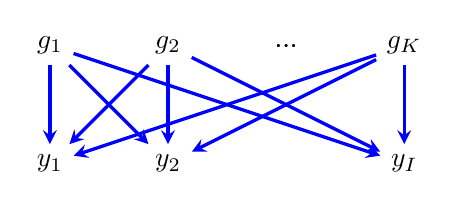
\begin{tikzpicture}[>=stealth, node distance=1.5cm]
			\tikzstyle{format} = [draw, thick, circle, minimum size=1.0mm, inner sep=0pt]
			\tikzstyle{square} = [draw, thick, minimum size=1.0mm, inner sep=3pt]

			\begin{scope}
			\path[->, very thick]

			node[] (g1) {$g_1$}
			node[right of=g1] (g2) {$g_2$}
			node[right of=g2] (lips) {$...$}
			node[right of=lips] (gn) {$g_K$}
			node[below of=g1] (y1) {$y_1$}
			node[below of=g2] (y2) {$y_2$}
			node[right of=g2] (lips2) {$...$}
			node[below of=gn] (yn) {$y_I$}

			(g1) edge[blue, ->] (y1)
			(g2) edge[blue, ->] (y1)
			(gn) edge[blue, ->] (y1)
			(g1) edge[blue, ->] (y2)
			(g2) edge[blue, ->] (y2)
			(gn) edge[blue, ->] (y2)
			(g1) edge[blue, ->] (yn)
			(g2) edge[blue, ->] (yn)
			(gn) edge[blue, ->] (yn)
			;
			\end{scope}

			\end{tikzpicture}
		}
	\end{center}
\end{figure}
This approach learns, for each gene $i$, a coefficient vector $\beta_i \in \mathcal{R}^K$, where $K$ is the total number of guides introduced to the pool. These coefficients are then used to cluster guides (and, more importantly, their transcription factor targets) into modules, and genes into programs.
\begin{figure}[H]
     \centering
     \begin{subfigure}[b]{0.48\textwidth}
         \centering
         \includegraphics[width=\textwidth]{no_ct_guide_hm.png}
         \caption{TFs targeted by guides that display similar effects are partitioned into modules}
				 \label{guide_clust}
     \end{subfigure}
     \hfill
     \begin{subfigure}[b]{0.48\textwidth}
         \centering
         \includegraphics[width=\textwidth]{guide_exp_hm.png}
         \caption{Similar to how TFs are clustered into modules, shown in (a), genes are also clustered based on their learned coefficients, into programs.}
         \label{guide_exp}
     \end{subfigure}
        \caption{Key results to replicate from Perturb-seq original paper}
        \label{fig:three graphs}
\end{figure}
They validated their results with ChIP-Seq data: the gene programs that they identified as regulated by TFs were enriched for genes that had been previously reported to be bound to (evidence for being regulated by) those same TFs in ChIP data. One other interesting result from the paper was that incorporation of an additional covariate, cell state, which was learned from unperturbed cells, reduced many of the correlations between guides.
\begin{figure}[H]
\centering
\includegraphics[width=0.5\textwidth]{ct_guide_hm.png}
\end{figure}
This suggests that many of the detected relationships stem from indirect rather than direct correlation. The authors also inferred a more complete regulatory network over just the transcription factors included in the study.
\begin{figure}[H]
\centering
\includegraphics[width=0.75\textwidth]{tf_net.png}
\end{figure}
\section*{Project Proposal}
In this project, I plan to
\begin{enumerate}
\item Replicate the subfigures shown above from figures 3 and 4 from the original Perturb-seq paper. I don't believe they provided a method for the learning of the TF GRN (D) from the correlation data (C), so if possible I'd like to leave this as a bonus rather than a requirement from my project, as it isn't the aspect of this work that I'd like to most focus on.
\item Test whether the conditional independences revealed by controlling for cell type are supported by the ChIP-seq data. For each TF targeted by a guide $g$, I will identify the genes $y$ who have an edge $g \diedgeright y$ in the model that does not control for cell type. I will then divide these genes into two groups, those that do and don't have an edge in the model that does control for cell type. My hypothesis is that the genes that lack an edge in the cell type control model will be less enriched for ChIP overlap, because these are not directly regulated by the TF ($y \ci g \mid s$, where $s$ is cell type). Cell type is not directly observed, so cell types are learned from unperturbed cells and then assigned to perturbed cells through the use of a classifier trained on the unperturbed cells.
\item In addition to binary guide nodes which suggest TF knockout, incorporate TF expression nodes as potential predictors in training MIMOSCA. In reality, I expect almost all guide-gene edges to be mediated by the transcription factor the guide is targeting, so we should find many cases where $y \ci g \mid y_{TF}$ (or $y \ci g \mid y_{TF}, s$, if the cell type control model did display the expected enrichment pattern from [2]. It's possible that guide presence is actually a more stable metric for TF expression than the directly measured expression that single-cell RNA-seq can provide, but I can directly look into this as a first step. It would be interesting to see whether we can obtain similar results with TF expression as a predictor. If we can't, it could just be reflective of the weaknesses of scRNA-seq (as just described), or it could also suggest that some of the guide effects are mediated by off-target binding of the guides rather than the expected regulatory relationships, or another unmodeled factor.
\end{enumerate}
\section*{Data Availability}
The data from the paper was available on GEO, and I've downloaded the perturbed expression data. I need to download the ChIP-Seq data, but the authors report it as available, and the perturbed expression data was very easy to find. I believe I have the unperturbed data, although it's not the most clearly labeled, so after I attempt cell type clustering, if this isn't what I expect, I may look into some of the alternative approaches that have recently been developed for identifying cell types directly from perturbed data, which could involve limiting the rest of the scope of the project, as that would take more time than I expect to attribute to obtain cell type assignments. I plan to produce all code from scratch - the authors have a github which is poorly commented and not too useful, and I am interested in fully understanding these methods.
\bibliographystyle{apalike}
\bibliography{references}






\end{document}
